\documentclass[exercice, a4]{thedocument}%
    \usepackage{texmaths-symbols}
    \usepackage{texmaths-tikz}
    \usepackage{scratch3}
    \usepackage{tabularx}
\startdatakeys
    \source{26GENMATAA1X}
    \BO{2026}
    \cycle{4}
    \competencesDuSocle{}
    \automatismes{B1db}
    \objectifsApprentissage{E1af, E1ae}
\enddatakeys
\begin{document}%
    \begin{minipage}{0.48\linewidth}
        \mathspoint{ABCD} est un carré.

        \mathspoint{ABF} est un triangle équilatéral.

        \mathspoint{AF} $= 4$ cm.

        Les points \mathspoint{F}, \mathspoint{A} et \mathspoint{E} sont alignés.
    \end{minipage}\hfill
    \begin{minipage}{0.48\linewidth}
        \begin{center}
            \begin{tikzpicture}[scale=0.85]
                \coordinate (F) at (0,0);
                \coordinate (A) at (4,0);
                \coordinate (E) at (8,0);
                \coordinate (B) at (2,3.46);
                \coordinate (C) at (5.46,5.46);
                \coordinate (D) at (7.46,2);
                
                \draw (F) -- (A) -- (B) -- cycle;
                \draw (A) -- (B) -- (C) -- (D) -- cycle;
                \draw[->] (A) -- (E);
                \draw (F) -- (A);
                
                \tkzMarkSegments[mark=s||](%
                    F,B B,C C,D A,D A,B F,A A,E%
                    )
                
                \node[left] at (F) {$F$};
                \node[below] at (A) {$A$};
                \node[right] at (E) {$E$};
                \node[above left] at (B) {$B$};
                \node[above] at (C) {$C$};
                \node[right] at (D) {$D$};
                \node[below] at (3,-0.3) {4 cm};
                
                \pic[
                    draw,
                    green!50!black,
                    angle radius=0.5cm,
                    angle eccentricity=1.6%
                    ] {angle = E--A--D};
            \end{tikzpicture}
        \end{center}
    \end{minipage}

    \begin{enumerate}
    \item Justifier que la mesure de l'angle $\widehat{\mathspoint{EAD}}$ est égale à $30^\circ$.

    Dans la suite de l'exercice on utilisera l'échelle suivante : \textbf{10 pas} dans le programme représentent \textbf{1 cm} dans la réalité.

    \item Le \textbf{bloc triangle} ci-dessous permet de tracer un triangle équilatéral et le \textbf{bloc carré} permet de construire un carré :

    \begin{center}
        \begin{tabular}{|p{7cm}|p{7cm}|}
            \hline
            \textbf{Le bloc triangle} & \textbf{Le bloc carré} \\
            \hline
            \begin{scratch}
            \initmoreblocks{définir \namemoreblocks{Triangle}}
            \blockrepeat{répéter \ovalnum{3} fois}
            {
            \blockmove{avancer de \ovalnum{\textbf{J}}}
            \blockmove{tourner \turnleft{} de \ovalnum{\textbf{K}} degrés}
            }
            \end{scratch}
            &
            \begin{scratch}
            \initmoreblocks{définir \namemoreblocks{Carré}}
            \blockrepeat{répéter \ovalnum{4} fois}
            {
            \blockmove{avancer de \ovalnum{\textbf{M}}}
            \blockmove{tourner \turnleft{} de \ovalnum{N} degrés}
            }
            \end{scratch}
            \\ \hline
        \end{tabular}
    \end{center}

    Donner les valeurs de \textbf{J}, \textbf{K}, \textbf{M} et \textbf{N} pour que les blocs triangle et carré permettent de construire un triangle équilatéral de 4 cm de côté et un carré de 4 cm de côté.

    \emph{Aucune justification n'est attendue.}

    \item Le \textbf{programme principal} utilise le bloc \textbf{Triangle} et le bloc \textbf{Carré}.

    L'instruction \guillemets{s'orienter à $90^\circ$} signifie que l'on s'oriente vers la droite.

    Écrire sur la copie le numéro de la figure obtenue grâce à ce programme.

    \emph{Aucune justification n'est attendue.}

    \end{enumerate}

\begin{tabularx}{.9\linewidth}{|m{8.9cm}|X|}\hline
\textbf{Figure 1}&\textbf{Programme principal}\\
\begin{tabular}{|m{8.5cm}|}
\hline
    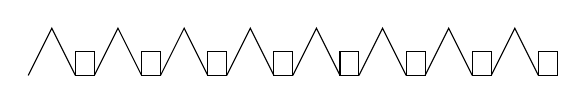
\begin{tikzpicture}[scale=0.6]
    \foreach \x in {0,...,7} {
     \draw (\x*1.4,0) -- (\x*1.4+0.5,1) -- (\x*1.4+1,0);
     \draw (\x*1.4+1,0) rectangle (\x*1.4+1.4,0.5);
    }
    \end{tikzpicture}
\\ \hline
\end{tabular}

\begin{tabular}{|m{3.75cm}|m{4.25cm}|}\hline
\textbf{Figure 2}&\textbf{Figure 3}\\
\begin{center}
    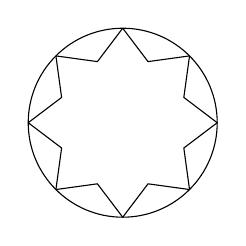
\begin{tikzpicture}[scale=0.6]
    \draw (0,0) circle (2);
    \foreach \i in {0,...,7} {
    \draw ({2*cos(45*\i)},{2*sin(45*\i)}) -- ({1.4*cos(45*\i+22.5)},{1.4*sin(45*\i+22.5)}) -- ({2*cos(45*\i+45)},{2*sin(45*\i+45)});
    }
    \end{tikzpicture}
\end{center}
&
\begin{center}
    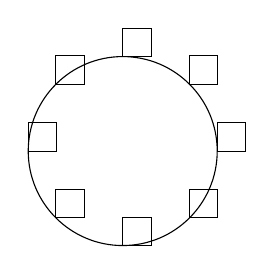
\begin{tikzpicture}[scale=0.6]
    \draw (0,0) circle (2);
    \foreach \i in {0,...,7} {
     \draw ({2*cos(45*\i)},{2*sin(45*\i)}) rectangle ++(0.6,0.6);
    }
    \end{tikzpicture}
\end{center}\\ \hline
\end{tabular}

\textbf{Figure 4}
    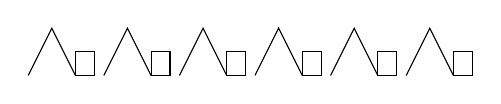
\begin{tikzpicture}[scale=0.6]
    \foreach \x in {0,...,5} {
    \draw (\x*1.6,0) -- (\x*1.6+0.5,1) -- (\x*1.6+1,0);
    \draw (\x*1.6+1,0) rectangle (\x*1.6+1.4,0.5);
    }
    \end{tikzpicture}
&
    \begin{center}
        \begin{scratch}[scale=1]
            \blockinit{quand \greenflag est cliqué}
            \blockmove{aller à x: \ovalnum{0} y: \ovalnum{-100}}
        \blockmove{s'orienter à \ovalnum{90}}
        \blockpen{effacer tout}
        \blockpen{stylo en position d'écriture}
        \blockrepeat{répéter \ovalnum{6} fois}
        {
            \blockmoreblocks{triangle}
            \blockmove{avancer de \ovalnum{50} pas}
            \blockmove{tourner \turnright{} de \ovalnum{30} degrés}
            \blockmoreblocks{Carré}
            \blockmove{avancer de \ovalnum{50} pas}
            \blockmove{tourner \turnleft{} de \ovalnum{30} degrés}
            }
        \end{scratch}
    \end{center}
        \\ 
        \hline
    \end{tabularx}
    \showthesource
    
    \end{document}